\documentclass[letterpaper,10pt,twocolumn,titlepage]{article}

\usepackage{graphicx}                                        
\usepackage{amssymb}                                         
\usepackage{amsmath}                                         
\usepackage{amsthm}                                          

\usepackage{alltt}                                           
\usepackage{float}
\usepackage{color}
\usepackage{url}

\usepackage{balance}
\usepackage[TABBOTCAP, tight]{subfigure}
\usepackage{enumitem}
\usepackage{pstricks, pst-node}

\usepackage{geometry}
\usepackage{listings}
\geometry{textheight=8.5in, textwidth=6in}

%random comment

\newcommand{\cred}[1]{{\color{red}#1}}
\newcommand{\cblue}[1]{{\color{blue}#1}}

\usepackage{hyperref}
\usepackage{geometry}

\def\name{Balaji Ramani}

%% The following metadata will show up in the PDF properties
\hypersetup{
  colorlinks = true,
  urlcolor = black,
  pdfauthor = {\name},
  pdfkeywords = {cs311 ``operating systems'' files filesystem
I/O},
  pdftitle = {CS 311 Project 3:},
  pdfsubject = {CS 311 Project 3},
  pdfpagemode = UseNone
}

\begin{document}
\title{CS311: Operating Systems I - Assignment 3}
\author{Balaji Ramani}
\date{Feb 10, 2012}
\maketitle


\section{Code Documentation}
	The entire logic is divided into two functions - main and cross\_off\_non\_primes.\newline
The main function is responsible for spawning threads and browse through the bitmap to collect all prime numbers and store it in an array. The main function also divides the entire range between zero and UINT\_MAX into multiple partitions. The number of partitions depends on the number of threads. The partition array doesn't contain all the numbers in its range but only the maximum value of the range. The partitions array is a global variable. Each spawned thread is responsible for its own partition.\newline
	The cross\_off\_non\_primes is the function that is executed by the spawned threads. The cross\_off\_non\_primes function browses through the bitmap and sets all the bits corresponding to a non-prime number to one.\newline
	The algorithm used here is Sieve of Eratosthenes as mentioned in wikipedia\newline
		a. Create a list of consecutive integers from 2 to n: (2, 3, 4, ..., n).\newline
		b. Initially, let p equal 2, the first prime number.\newline
		c. Starting from p, count up in increments of p and mark each of these numbers greater than p itself in the list. These numbers will be 2p, 3p, 4p, etc.; note that some of them may have already been marked.\newline
		d. Find the first number greater than p in the list that is not marked; let p now equal this number (which is the next prime).\newline
		e. If there were no more unmarked numbers in the list, stop. Otherwise, repeat from step 3.\newline
		f. When the algorithm terminates, all the numbers in the list that are not marked are prime.\newline
		g. As a refinement, it is sufficient to mark the numbers in step 3 starting from p2, as all the smaller multiples of p will have already been marked at that point. This means that the algorithm is allowed to terminate in step 5 when p2 is greater than n.\newline
		h. Another refinement is to initially list odd numbers only, (3, 5, ..., n), and count up using an increment of 2p in step 3, thus marking only odd multiples of p greater than p itself. This actually appears in the original algorithm. This can be generalized with wheel factorization, forming the initial list only from numbers coprime with the first few primes and not just from odds, i.e. numbers coprime with 2.\newline


\section{Commit logs}
  \begin{tabular}{ | l | l |}
    \hline
    Time & Message\\ \hline
2012/02/27 23:20 & graphs \\ \hline
2012/02/27 16:02 & adding doc.tex and some more changes to finding\_primes.c \\ \hline
2012/02/27 15:47 & adding comments \\ \hline
2012/02/27 15:35 & fixed infinite loop issue \\ \hline
2012/02/24 01:27 & fixed segfault error \\ \hline
2012/02/23 00:59 & thread function that crosses off non-primes \\ \hline
2012/02/20 21:30 & fixed few errors \\ \hline
2012/02/20 10:10 & initialize commit \\ \hline
  \end{tabular}

\begin{figure}
	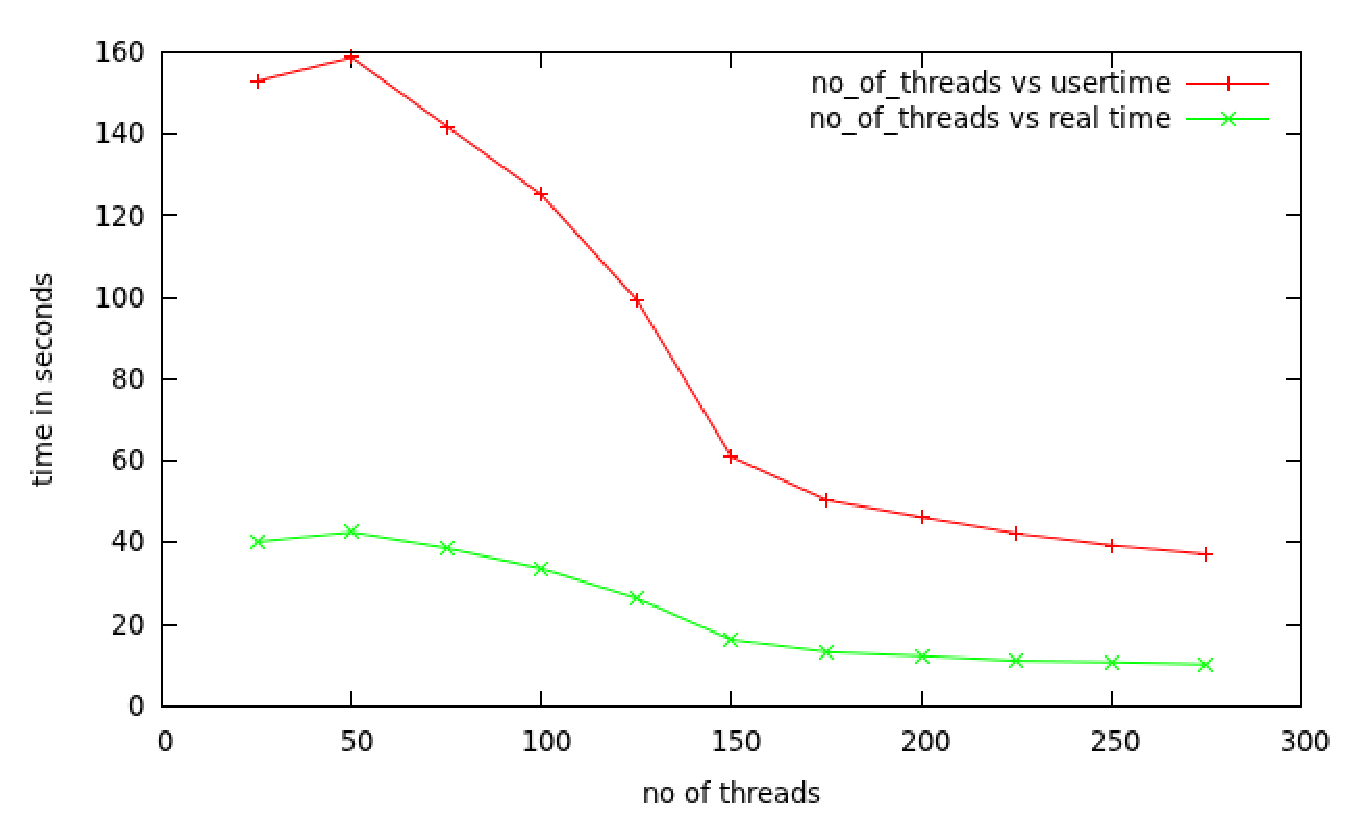
\includegraphics[scale=0.5]{graph-1.eps}
\end{figure}
\begin{figure}
	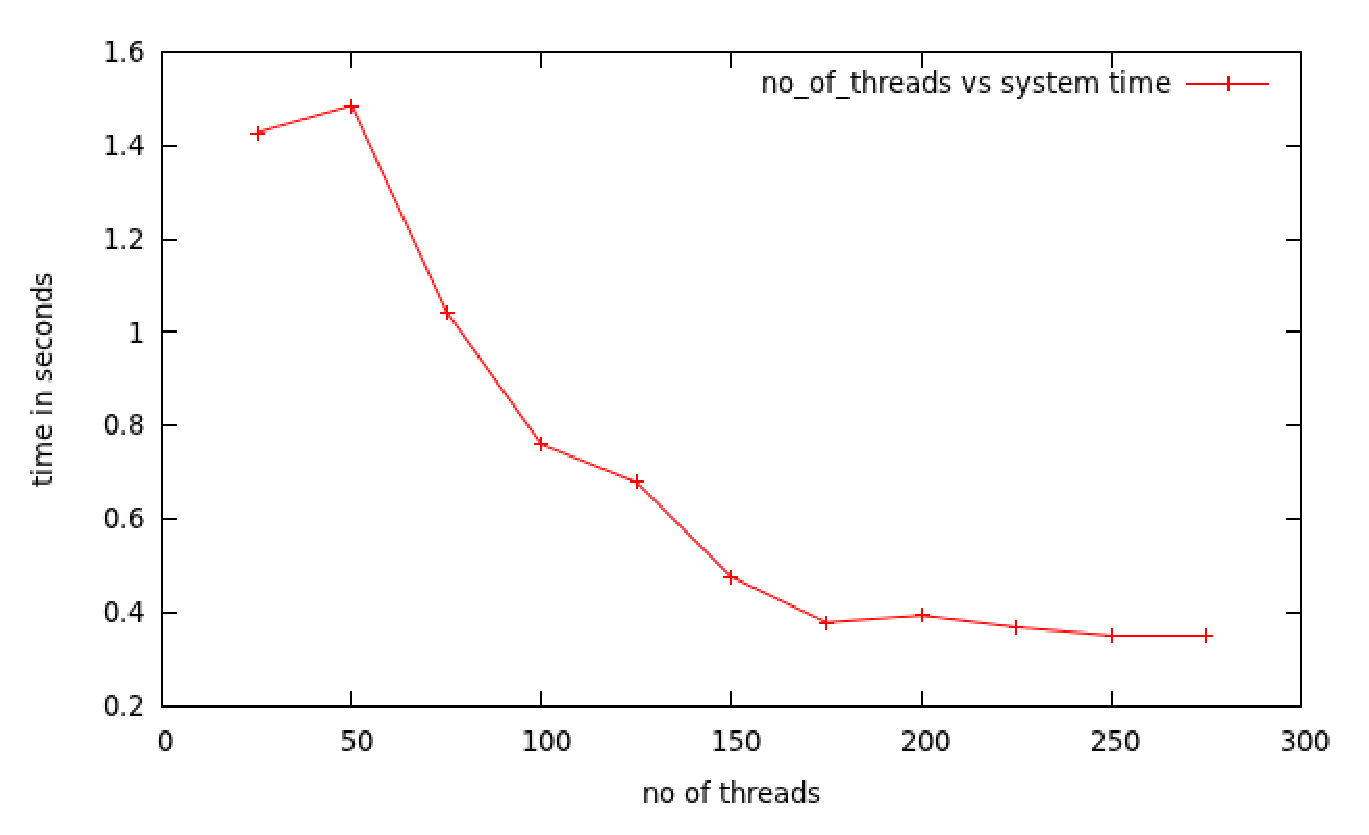
\includegraphics[scale=0.5]{graph-2.eps}
\end{figure}
\end{document}
